\documentclass[tikz,border=10pt]{standalone}
\usepackage{amsmath}
\begin{document}
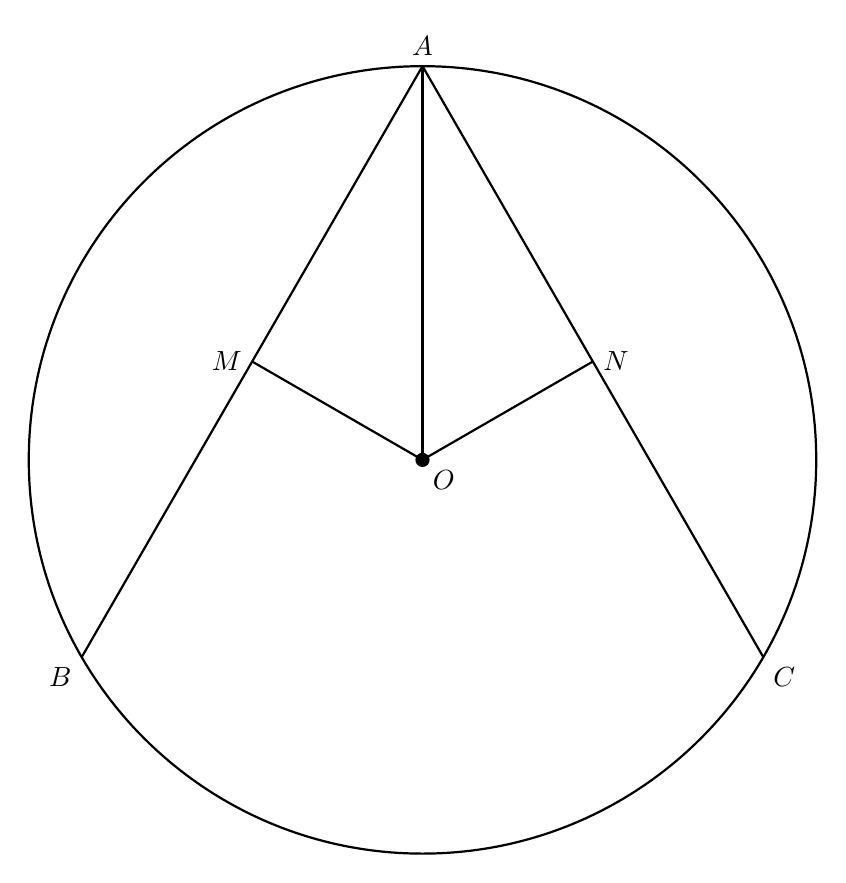
\begin{tikzpicture}[scale=0.05, line width=0.8pt]
  % Circle center O and radius
  \coordinate (O) at (0,0);
  \coordinate (A) at (0,100);
  \coordinate (B) at (-86.5,-50);
  \coordinate (C) at (86.5,-50);
  \coordinate (M) at (-43.3,25);
  \coordinate (N) at (43.3,25);

  % Circle
  \draw (O) circle (100);

  % Triangle sides and inner segments
  \draw (A) -- (B);
  \draw (A) -- (C);
  \draw (A) -- (O);
  \draw (M) -- (O);
  \draw (O) -- (N);

  % Points
  \fill (O) circle (1.8);
  \node[above] at (A) {$A$};
  \node[left] at (M) {$M$};
  \node[right] at (N) {$N$};
  \node[below left] at (B) {$B$};
  \node[below right] at (C) {$C$};
  \node[below right] at (O) {$O$};
\end{tikzpicture}
\end{document}
